\documentclass[review]{elsarticle}

\usepackage{amsmath}
\usepackage{booktabs}
\usepackage{dirtytalk}
\usepackage{subcaption}
\usepackage{tabularx}
\usepackage{nicefrac}
\usepackage[usenames]{xcolor}
\usepackage{lineno,hyperref}
\modulolinenumbers[5]

\journal{Composites Part A}

%%%%%%%%%%%%%%%%%%%%%%%
%% Elsevier bibliography styles
%%%%%%%%%%%%%%%%%%%%%%%
%% To change the style, put a % in front of the second line of the current style and
%% remove the % from the second line of the style you would like to use.
%%%%%%%%%%%%%%%%%%%%%%%

%% Numbered
%\bibliographystyle{model1-num-names}

%% Numbered without titles
%\bibliographystyle{model1a-num-names}

%% Harvard
%\bibliographystyle{model2-names.bst}\biboptions{authoryear}

%% Vancouver numbered
%\usepackage{numcompress}\bibliographystyle{model3-num-names}

%% Vancouver name/year
%\usepackage{numcompress}\bibliographystyle{model4-names}\biboptions{authoryear}

%% APA style
%\bibliographystyle{model5-names}\biboptions{authoryear}

%% AMA style
%\usepackage{numcompress}\bibliographystyle{model6-num-names}

%% `Elsevier LaTeX' style
\bibliographystyle{elsarticle-num}
%%%%%%%%%%%%%%%%%%%%%%%

\begin{document}

\begin{frontmatter}

\title{Clusters}
%\tnotetext[mytitlenote]{Fully documented templates are available in the elsarticle package on \href{http://www.ctan.org/tex-archive/macros/latex/contrib/elsarticle}{CTAN}.}

%% Group authors per affiliation:
%\author{Luca Di Stasio\fnref{myfootnote}}
%\address{Radarweg 29, Amsterdam}
%\fntext[myfootnote]{Since 1880.}

%% or include affiliations in footnotes:
\author[lulea]{Luca Di Stasio}
\author[lulea]{Janis Varna}
%\ead[url]{www.elsevier.com}

%\author[mysecondaryaddress]{Global Customer Service\corref{mycorrespondingauthor}}
%\cortext[mycorrespondingauthor]{Corresponding author}
%\ead{support@elsevier.com}

\address[lulea]{Lule\aa\ University of Technology, University Campus, SE-97187 Lule\aa, Sweden}

\begin{abstract}
\noindent

\end{abstract}

\begin{keyword}
Polymer-matrix Composites (PMCs)\sep Transverse Failure \sep Debonding \sep Finite Element Analysis (FEA)
\end{keyword}


\end{frontmatter}

\linenumbers

%%%%%%%%%%%%%%%%%%%%%%%%%%%%%%%%%%%%%%%%%%%%%%%%%%%%%%%%%
%  INTRODUCTION
%%%%%%%%%%%%%%%%%%%%%%%%%%%%%%%%%%%%%%%%%%%%%%%%%%%%%%%%%

\section{Introduction}



%%%%%%%%%%%%%%%%%%%%%%%%%%%%%%%%%%%%%%%%%%%%%%%%%%%%%%%%%
%  RVE MODELS AND FE DISCRETIZATION
%%%%%%%%%%%%%%%%%%%%%%%%%%%%%%%%%%%%%%%%%%%%%%%%%%%%%%%%%

\section{RVE models \& FE discretization}

\subsection{Introduction \& Nomenclature}\label{subsec:names}



\subsection{Models of Representative Volume Element (RVE) and equivalent boundary conditions}\label{subsec:rve}



\begin{figure}[!h]
\centering
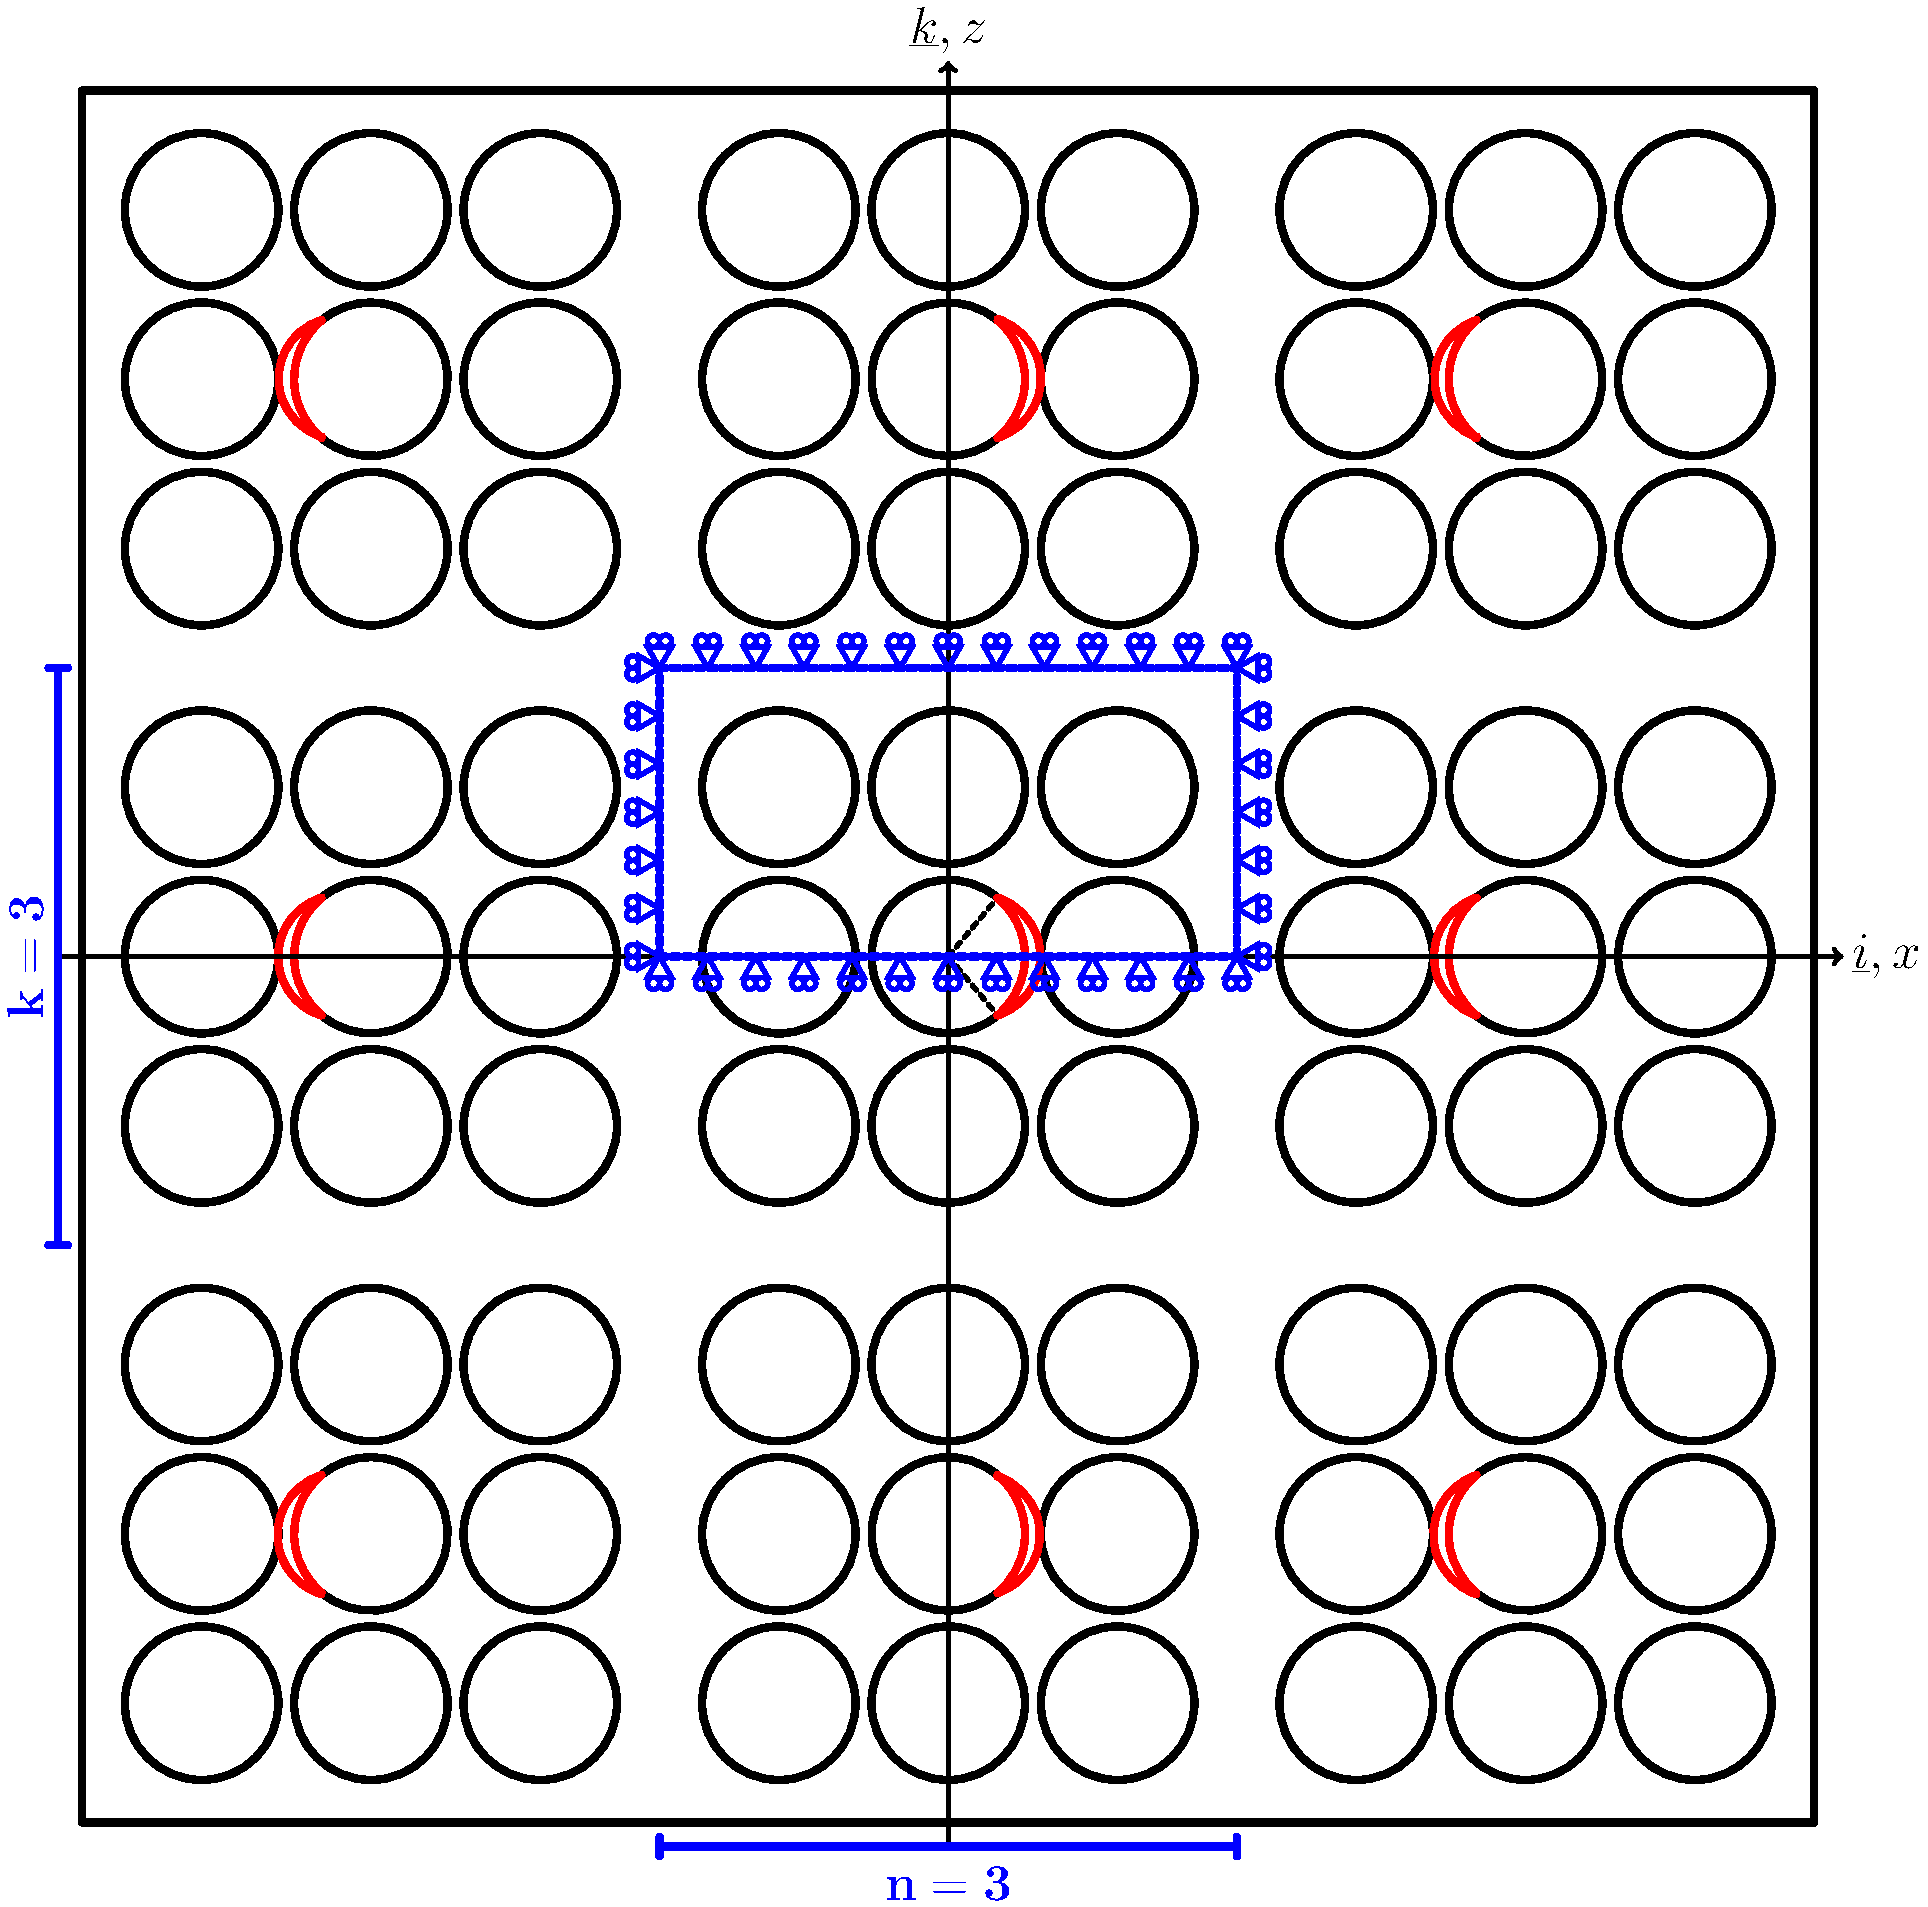
\includegraphics[width=\textwidth]{rveCoupling.pdf}
\caption{Models $n\times k-coupling$ with clusters.}\label{fig:laminateModelsA}
\end{figure}



\subsection{Finite Element (FE) discretization}

Discretization and analysis of RUCs is performed with the Finite Element Method (FEM) within the Abaqus environment, a commercial FEM software~\cite{abq12}. Length $l$ and height $h$ of the model are respectively determined by the number of fibers $n$ in the horizontal direction and $k$ across the thickness (see Sec.~\ref{subsec:rve}) according to Eq.~\ref{eq:lengthheight}:

\begin{equation}\label{eq:lengthheight}
l=2nL\qquad h=kL;
\end{equation}

where $2L$ is the length of a one-fiber unit, see Fig.~\ref{fig:modelschem}, and $L$ is defined as a function of the fiber volume fraction $V_{f}$ and the fiber radius $R_{f}$ according to

\begin{equation}\label{eq:LVf}
L=\frac{R_{f}}{2}\sqrt{\frac{\pi}{V_{f}}}.
\end{equation}

$R_{f}$ is assumed to be the same for every fiber and equal to $1\ \mu m$. The choice of the previous value is not dictated by physical considerations but for simplicity. It is thus useful to remark here that, in a linear elastic solution as the one considered in the present work, the ERR is proportional to the geometrical dimensions of the model and, consequently, recalculation of the ERR for fibers of any size requires a simple multiplication. Notice also that relationships in Eqs.~\ref{eq:lengthheight} and~\ref{eq:LVf} imply that the local and global $V_{f}$ are everywhere equal.

\begin{figure}[!h]
\centering
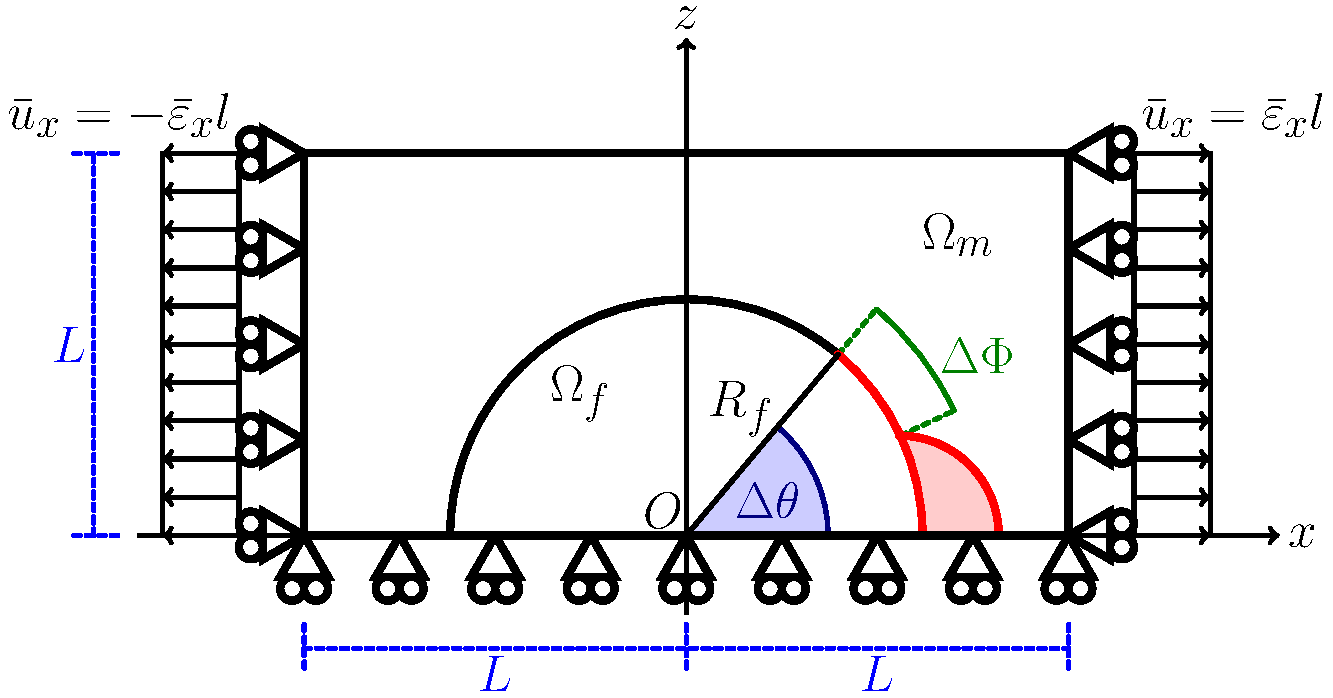
\includegraphics[width=\textwidth]{RUC.pdf}
\caption{Schematic of the model with its main parameters.}\label{fig:modelschem}
\end{figure}

The debond is placed symmetrically with respect to the $x$ axis (see Fig.~\ref{fig:modelschem}) and it is characterized by an angular size of $\Delta\theta$ (making the full debond size equal to $2\Delta\theta$). For large debond sizes (at least $\geq 60^{\circ}-80^{\circ}$), a region $\Delta\Phi$ of variable size appears at the crack tip where the crack faces are in contact with each other but free to slide relatively to each other. In order to model crack faces motion in the contact zone, frictionless contact is considered between the two crack faces to allow free sliding and avoid interpenetration. Symmetry with respect to the $x$ axis is applied on the lower boundary and coupling of vertical displacement on the upper boundary. Kinematic coupling on the $x$-displacement is applied along the left and right sides of the RUC in the form of a constant $x$-displacement $\pm\bar{\varepsilon}_{x} l$, corresponding to transverse strain $\bar{\varepsilon}_{x}$ equal to $1\%$.

\begin{table}[!htbp]
 \centering
 \caption{Summary of the mechanical properties of fiber and matrix. $E$ stands for Young's modulus, $\mu$ for shear modulus and $\nu$ for Poisson's ratio.}
 \begin{tabular}{cccc}
\textbf{Material} & \textbf{$E\left[GPa\right]$}\ & \textbf{$\mu\left[GPa\right]$} & \textbf{$\nu\left[-\right]$} \\
\midrule
Glass fiber    & 70.0  & 29.2   & 0.2  \\
Epoxy    & 3.5    & 1.25   & 0.4
\end{tabular}
\label{tab:phaseprop}
\end{table}

Meshing of the model is accomplished with second order, 2D, plane strain triangular (CPE6) and quadrilateral (CPE8) elements. A regular mesh of 8-node ($2^{nd}$ order rectangular) elements with almost unitary aspect ratio is enforced at the crack tip in order to ensure the convergence of the ERR. The angular size $\delta$ of an element in the crack tip neighborhood is always equal to $0.05^{\circ}$. The crack faces are modeled as element-based surfaces and a small-sliding contact pair interaction with no friction is imposed between them. The Mode I, Mode II and total Energy Release Rates (ERRs) (respectively referred to as $G_{I}$, $G_{II}$ and $G_{TOT}$) are the main result of FEM simulations; they are evaluated using the VCCT~\cite{Krueger2004} implemented in a in-house Python routine and, for $G_{TOT}$ only, the J-integral~\cite{Rice1968} is calculated by use of the Abaqus built-in command. A glass fiber-epoxy UD composite is treated in the present work, and it is assumed that their response lies always in the linear elastic domain. The material properties of glass fiber and epoxy are reported in Table~\ref{tab:phaseprop}. Validation is performed with respect to the results reported in~\cite{Paris2007,Sandino2016}, which were obtained with the Boundary Element Method (BEM) for a model of a single fiber with a symmetric debond placed in an infinite matrix. As discussed in more detail in~\cite{DiStasio2019}, the agreement between FEM (present work) and BEM~\cite{Paris2007,Sandino2016} solutions is good and the difference between the two does not exceed $5\%$. This provides us with a level of uncertainty with which we can analyze the significance of observed trends: any relative difference in ERR between different RUCs smaller than $5\%$ cannot be reliably distinguished from numerical uncertainty and its discussion should thus be avoided.

\section{Results \& Discussion}

\subsection{Coupling}\label{subsec:coupling}

\begin{figure}[!h]
\centering
    \begin{subfigure}[b]{0.475\textwidth}
        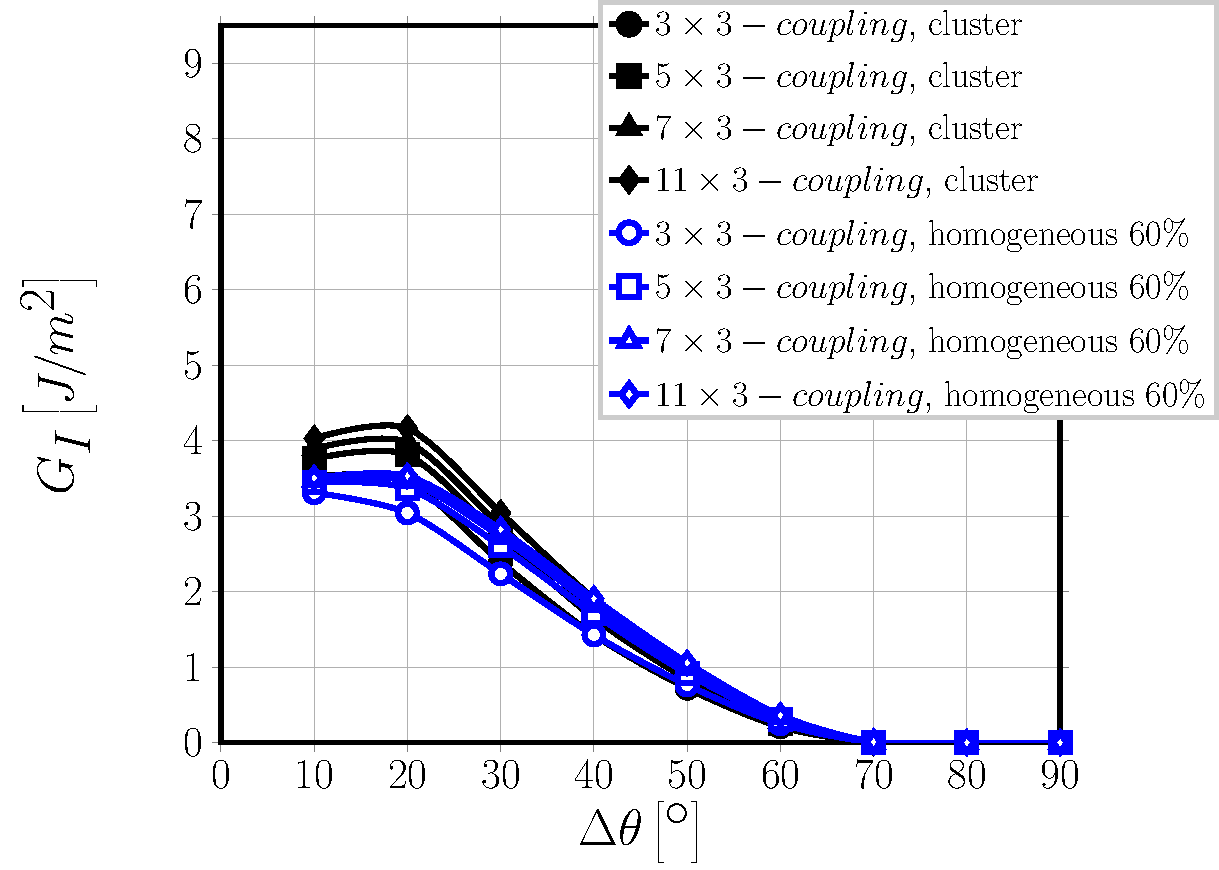
\includegraphics[width=\textwidth]{nx1-coupling-vf60-GI.pdf}
        \caption{Comparison with homogeneous RVE with $V_{f}=60\%$.}\label{subfig:clusterCouplingModeI60}
    \end{subfigure}\quad
    \begin{subfigure}[b]{0.475\textwidth}
        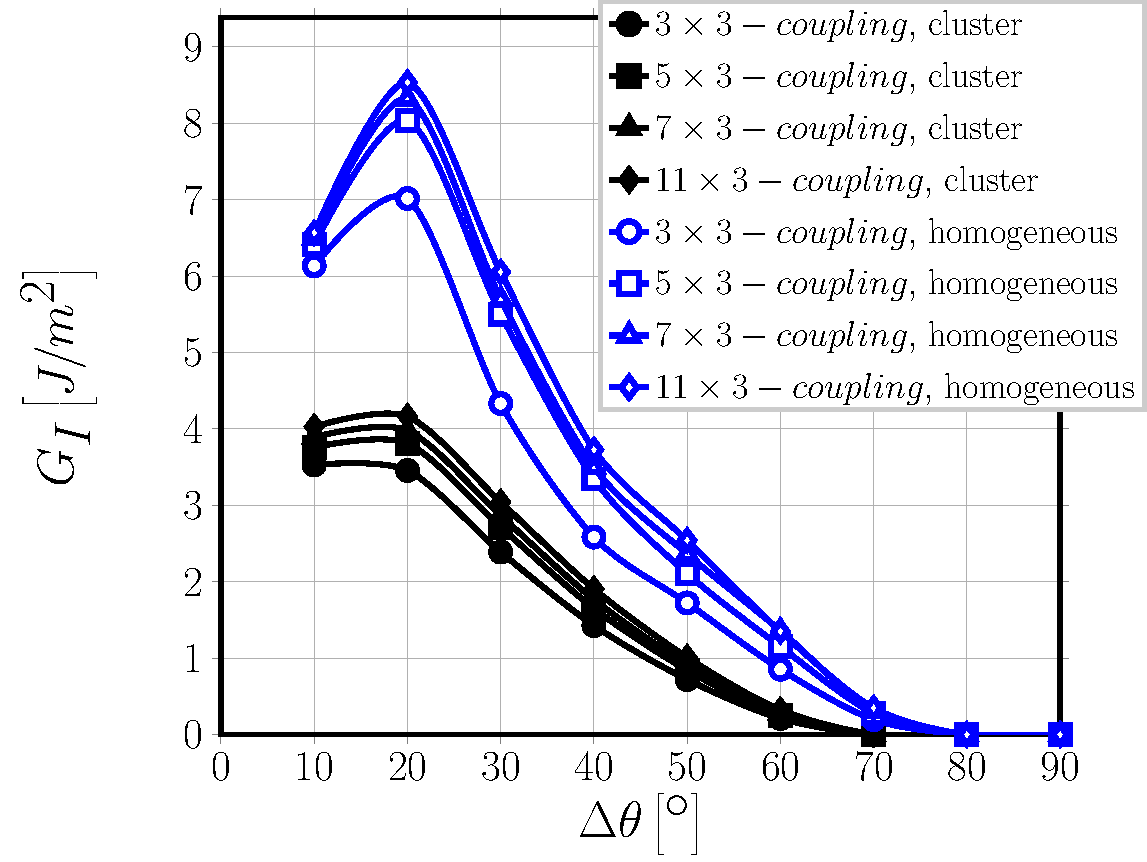
\includegraphics[width=\textwidth]{nx1-coupling-vf70-GI.pdf}
        \caption{Comparison with homogeneous RVE with $V_{f}=70\%$.}\label{subfig:clusterCouplingModeI70}
    \end{subfigure}

\caption{Effect of clustering on Mode I ERR in $n\times 1-coupling$ models. $V^{average}_{f}=60\%$, $V^{cluster}_{f}=70\%$, $\varepsilon_{x}=1\%$.}\label{fig:clusterCouplingModeI}
\end{figure}

\begin{figure}[!h]
\centering
    \begin{subfigure}[b]{0.475\textwidth}
        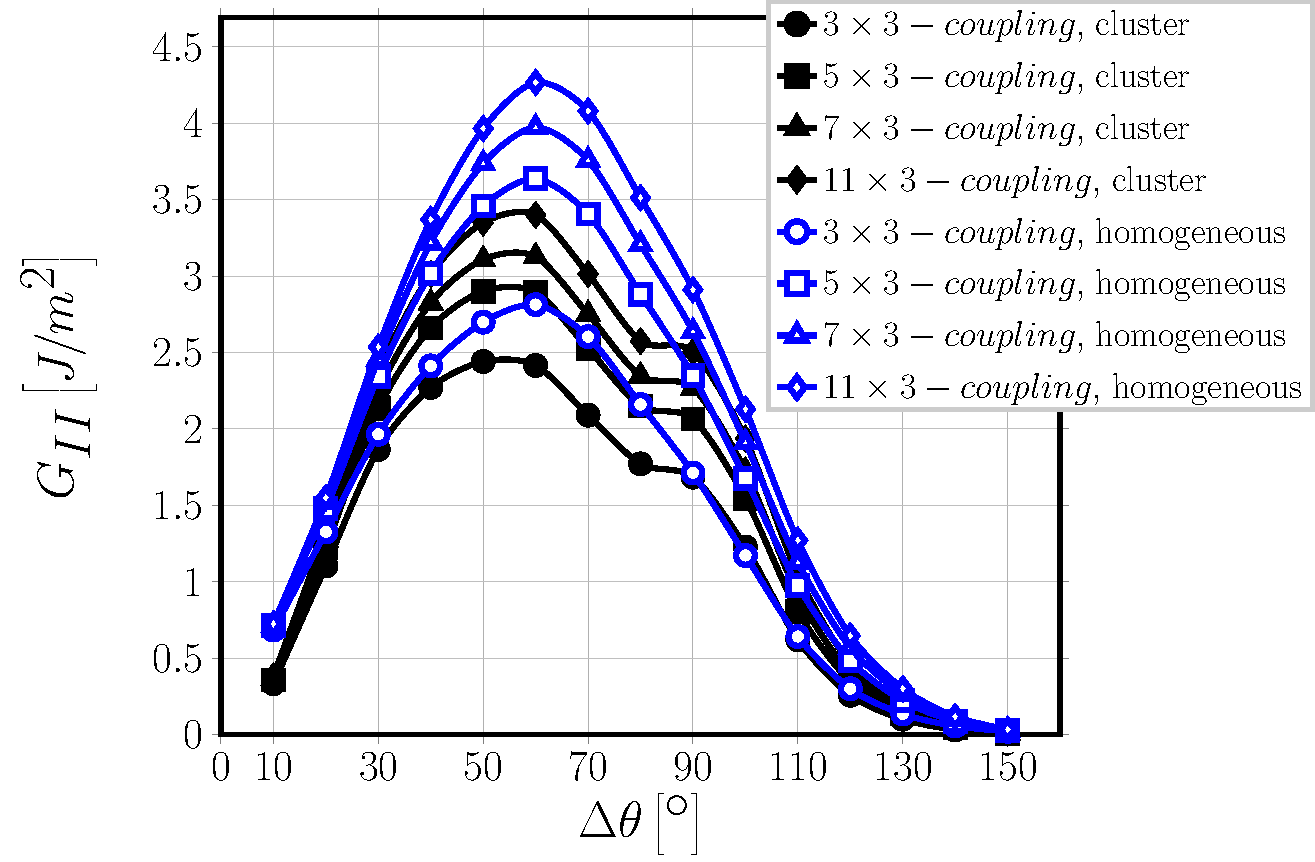
\includegraphics[width=\textwidth]{nx1-coupling-vf60-GII.pdf}
        \caption{Comparison with homogeneous RVE with $V_{f}=60\%$.}\label{subfig:clusterCouplingModeII60}
    \end{subfigure}\quad
    \begin{subfigure}[b]{0.475\textwidth}
        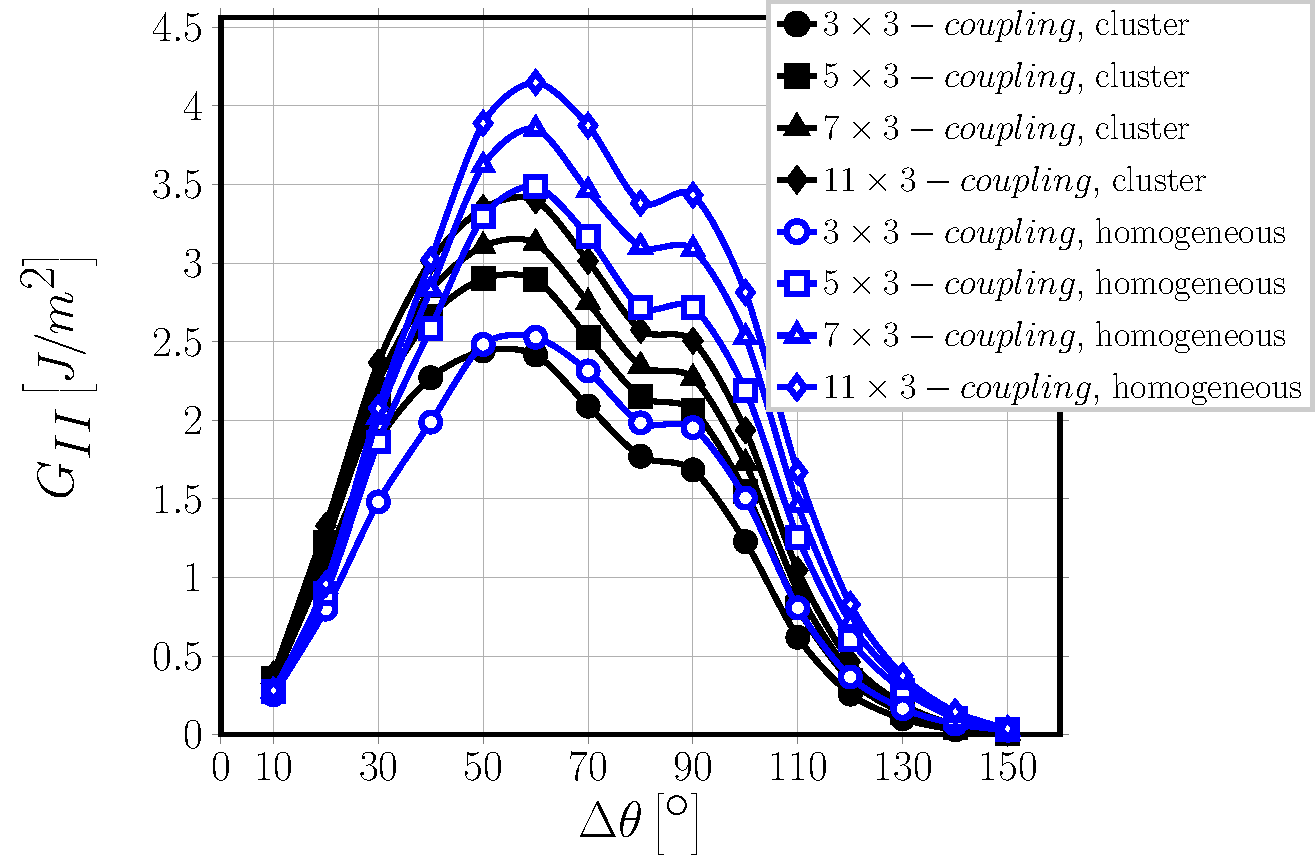
\includegraphics[width=\textwidth]{nx1-coupling-vf70-GII.pdf}
        \caption{Comparison with homogeneous RVE with $V_{f}=70\%$.}\label{subfig:clusterCouplingModeII70}
    \end{subfigure}

\caption{Effect of clustering on Mode II ERR in $n\times 1-coupling$ models. $V^{average}_{f}=60\%$, $V^{cluster}_{f}=70\%$, $\varepsilon_{x}=1\%$.}\label{fig:clusterCouplingModeI}
\end{figure}

\begin{figure}[!h]
\centering
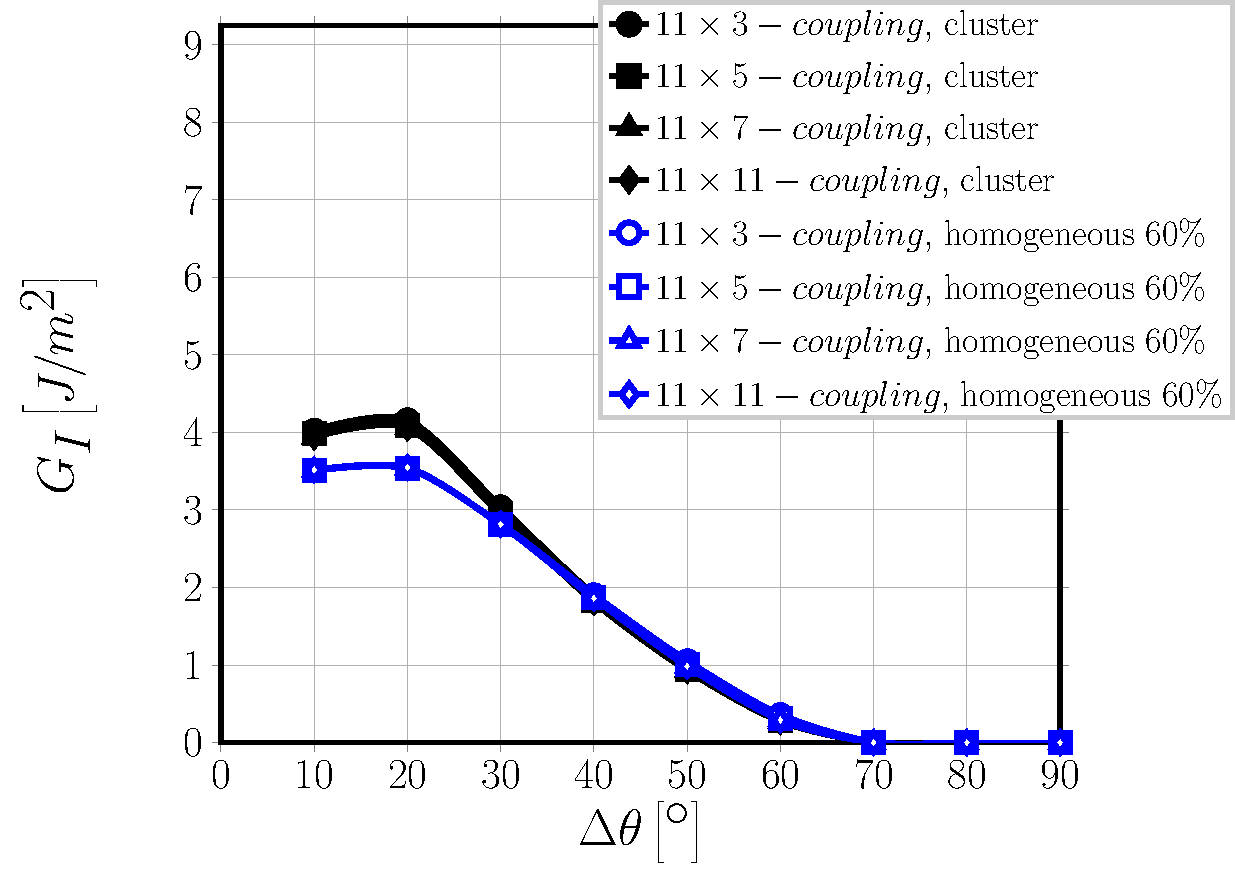
\includegraphics[width=\textwidth]{11xk-coupling-vf60-GI.pdf}
\caption{Clustering: models $11\times k-coupling$. $V_{f}=60\%$, $\varepsilon_{x}=1\%$.}\label{fig:debonddebondGI}
\end{figure}

\begin{figure}[!h]
\centering
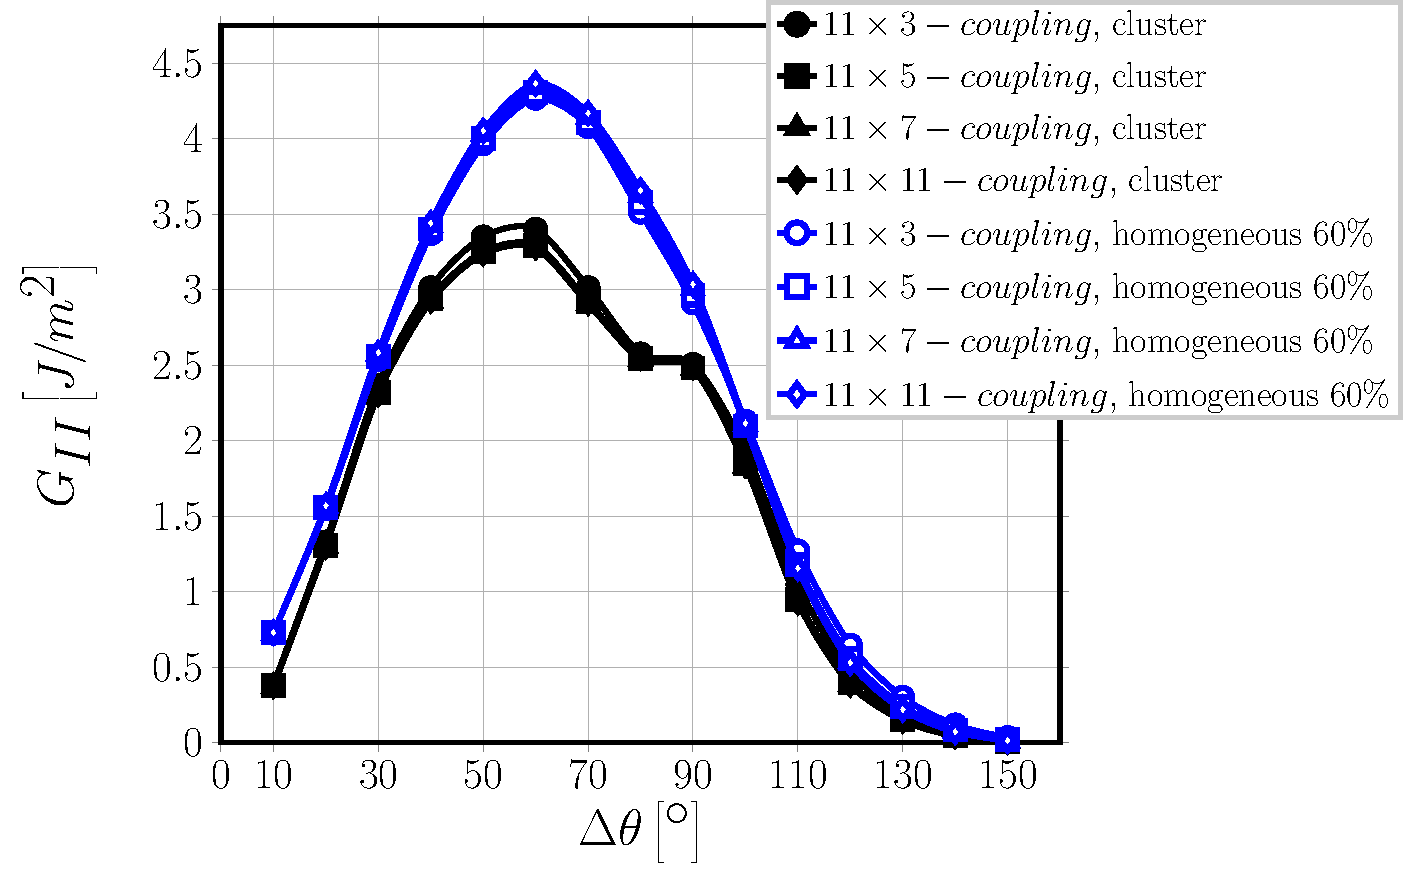
\includegraphics[width=\textwidth]{11xk-coupling-vf60-GII.pdf}
\caption{Clustering: models $11\times k-coupling$. $V_{f}=60\%$, $\varepsilon_{x}=1\%$.}\label{fig:debonddebondGI}
\end{figure}

\begin{figure}[!h]
\centering
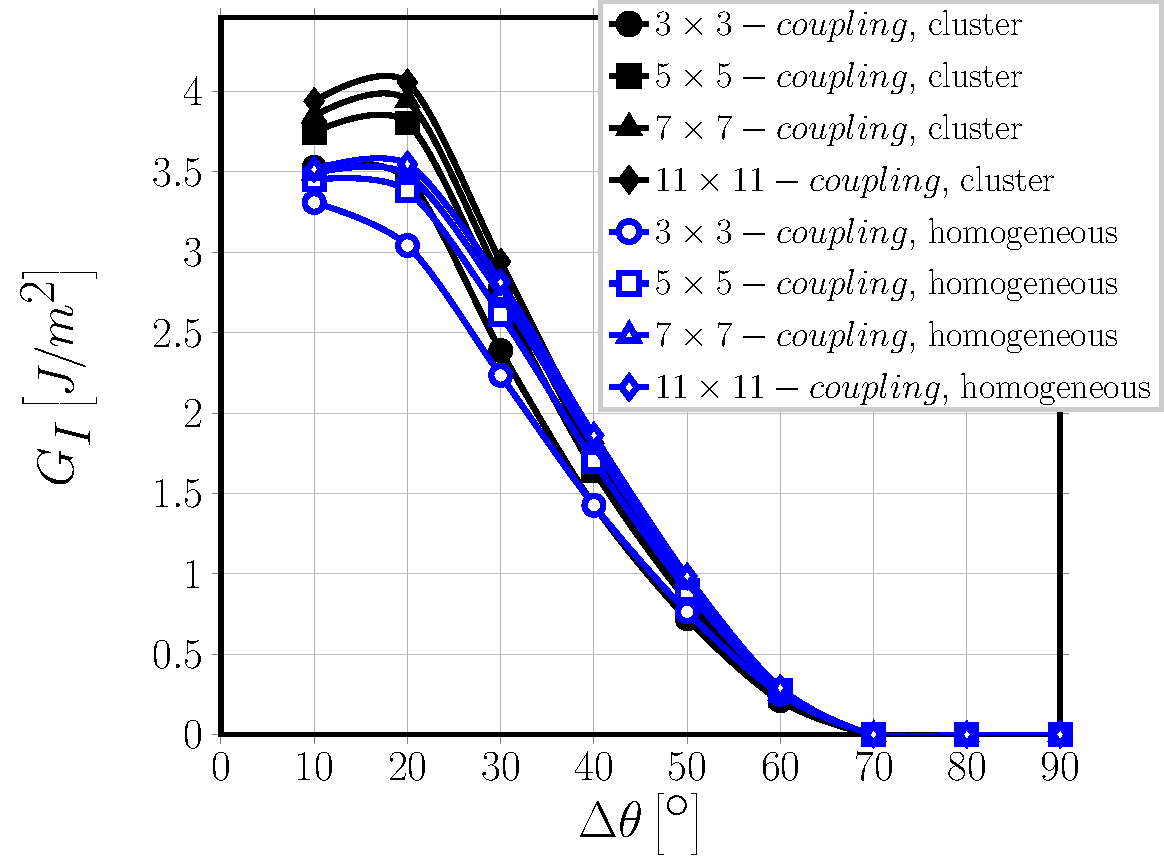
\includegraphics[width=\textwidth]{nxn-coupling-vf60-GI.pdf}
\caption{Clustering: models $n\times n-coupling$. $V_{f}=60\%$, $\varepsilon_{x}=1\%$.}\label{fig:debonddebondGI}
\end{figure}

\begin{figure}[!h]
\centering
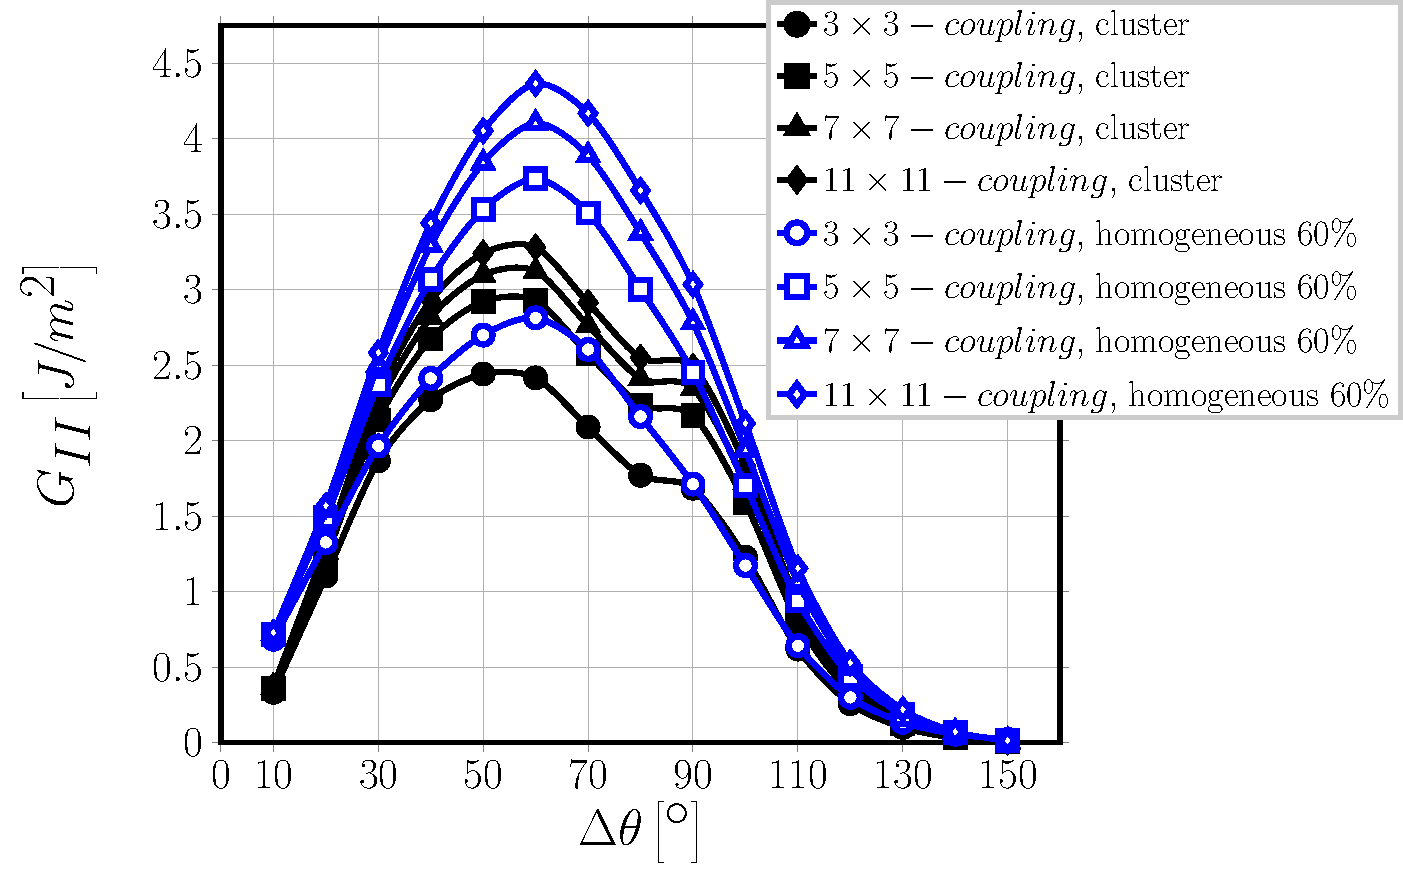
\includegraphics[width=\textwidth]{nxn-coupling-vf60-GII.pdf}
\caption{Clustering: models $n\times n-coupling$. $V_{f}=60\%$, $\varepsilon_{x}=1\%$.}\label{fig:debonddebondGI}
\end{figure}

\subsection{Cross-ply}\label{subsec:crossply}


\begin{figure}[!h]
\centering
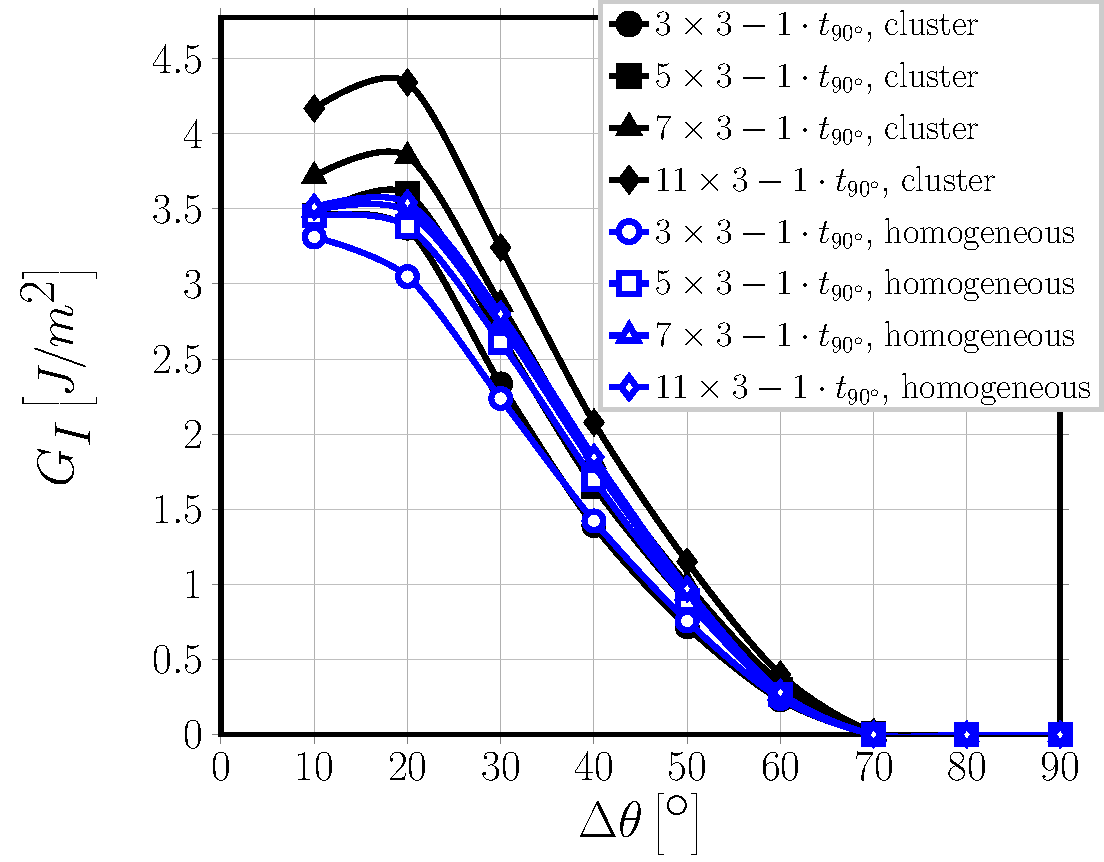
\includegraphics[width=\textwidth]{nx1-1t90-vf60-GI.pdf}
\caption{Clustering: models $n\times 1-1\cdot t_{90^{\circ}}$. $V_{f}=60\%$, $\varepsilon_{x}=1\%$.}\label{fig:debonddebondGI}
\end{figure}

\begin{figure}[!h]
\centering
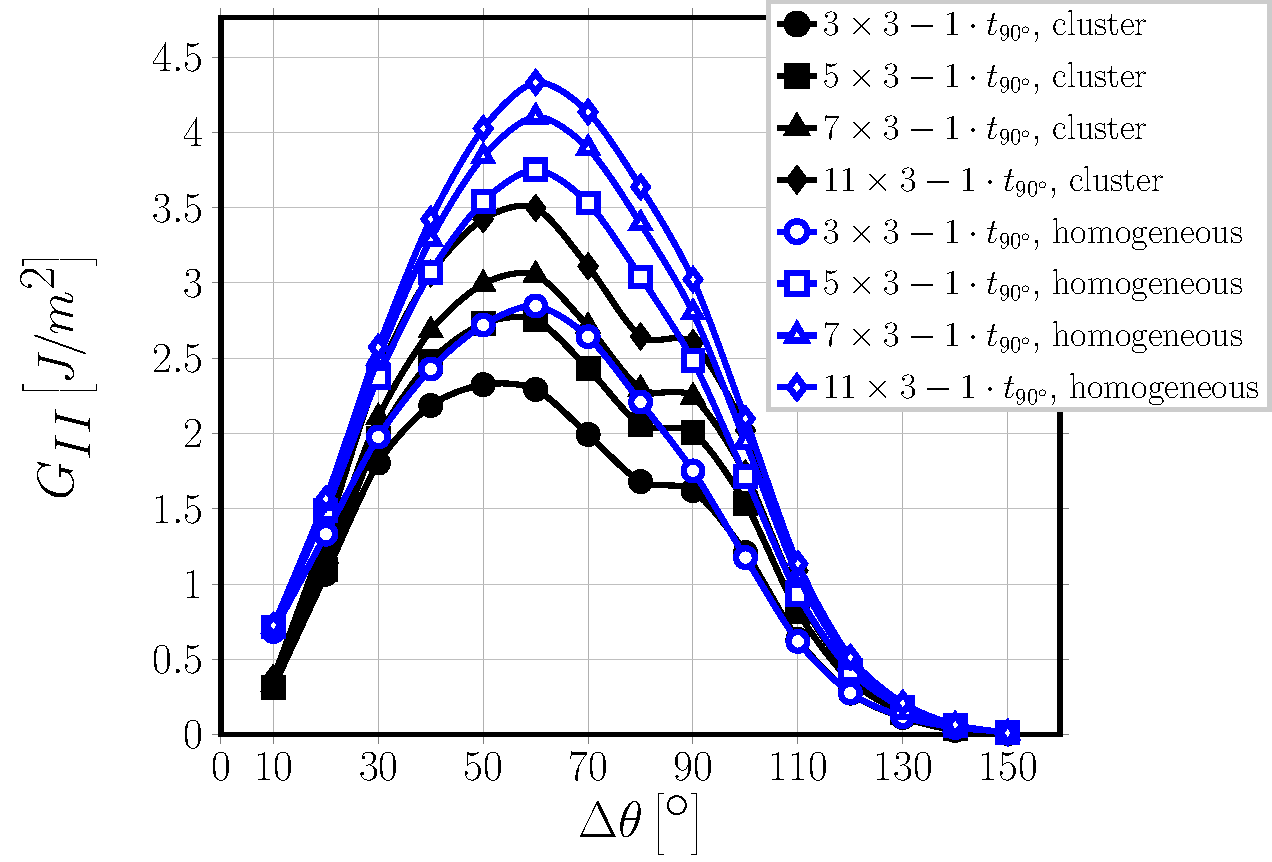
\includegraphics[width=\textwidth]{nx1-1t90-vf60-GII.pdf}
\caption{Clustering: models $n\times 1-1\cdot t_{90^{\circ}}$. $V_{f}=60\%$, $\varepsilon_{x}=1\%$.}\label{fig:debonddebondGI}
\end{figure}

\begin{figure}[!h]
\centering
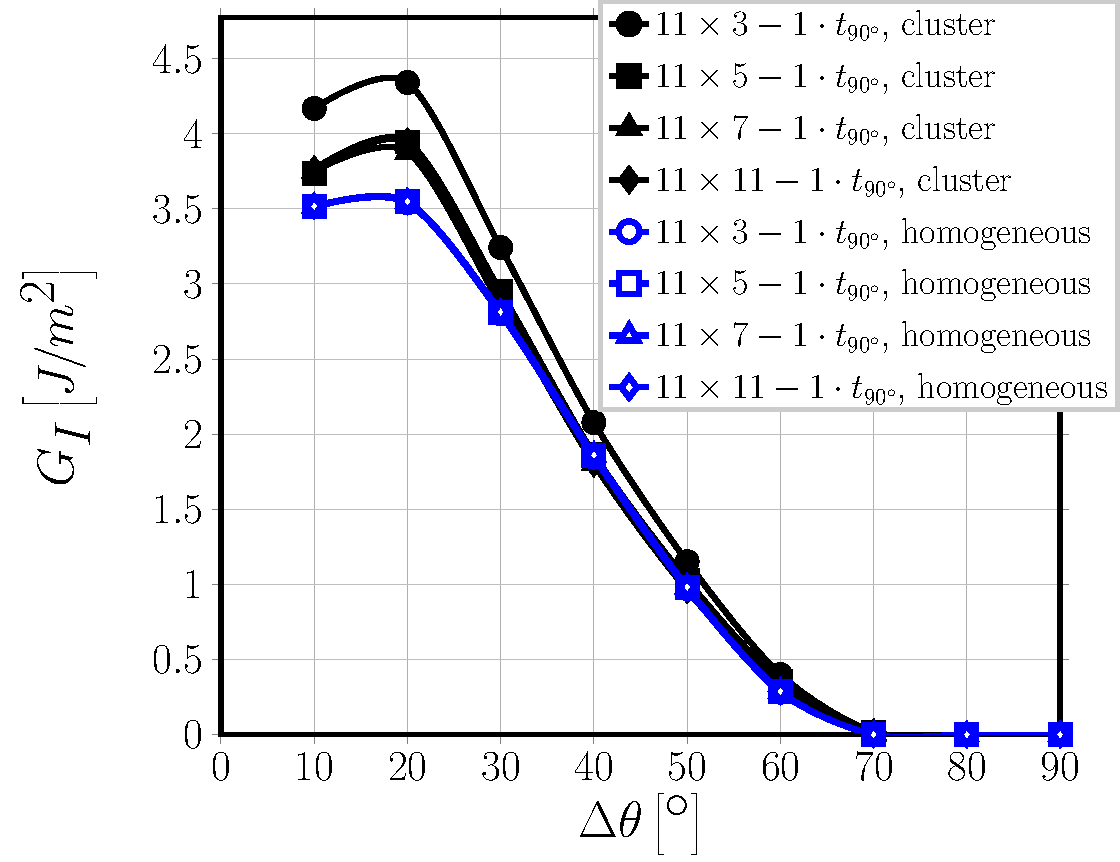
\includegraphics[width=\textwidth]{11xk-1t90-vf60-GI.pdf}
\caption{Clustering: models $11\times k-1\cdot t_{90^{\circ}}$. $V_{f}=60\%$, $\varepsilon_{x}=1\%$.}\label{fig:debonddebondGI}
\end{figure}

\begin{figure}[!h]
\centering
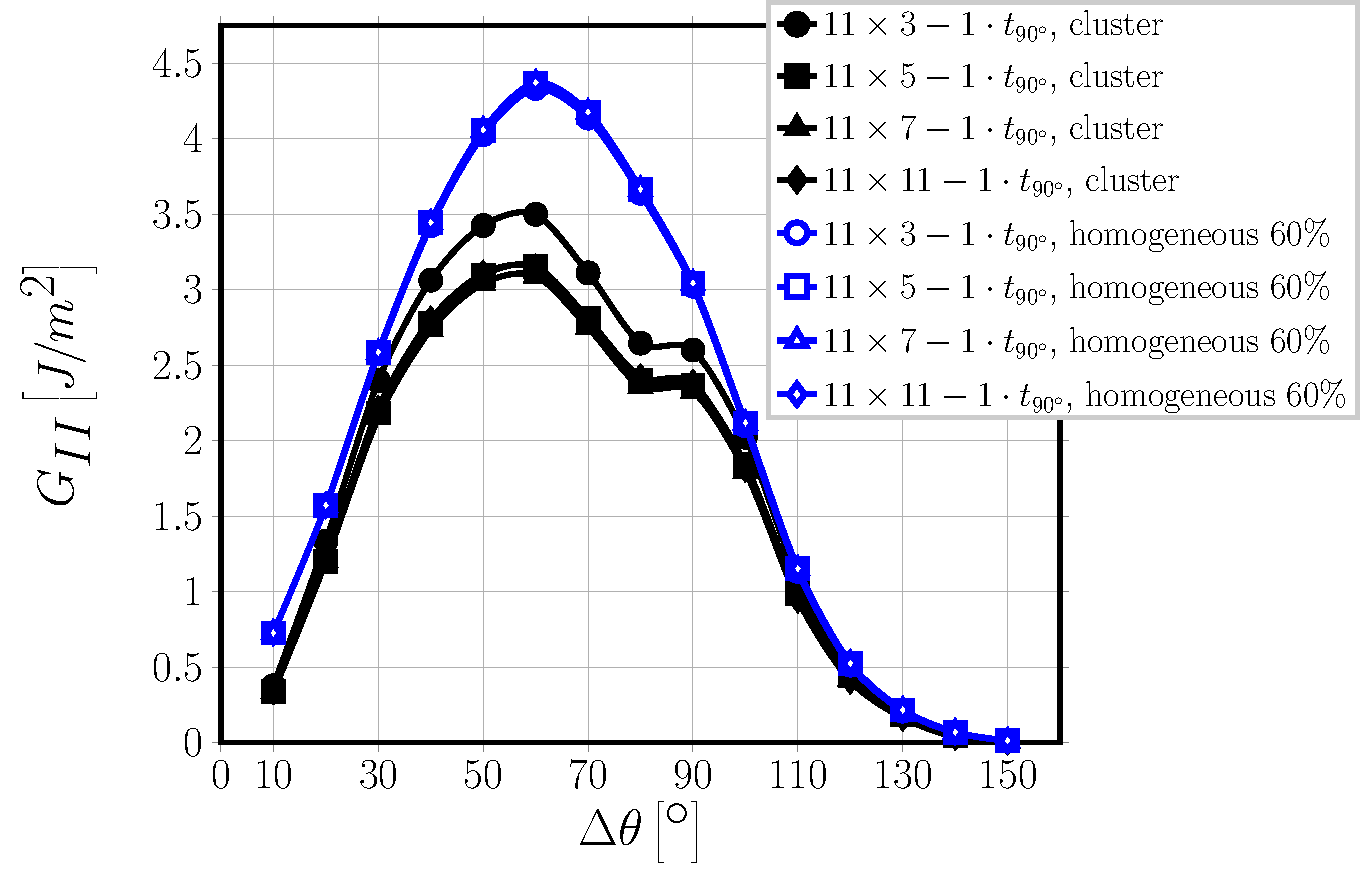
\includegraphics[width=\textwidth]{11xk-1t90-vf60-GII.pdf}
\caption{Clustering: models $11\times k-1\cdot t_{90^{\circ}}$. $V_{f}=60\%$, $\varepsilon_{x}=1\%$.}\label{fig:debonddebondGI}
\end{figure}

\begin{figure}[!h]
\centering
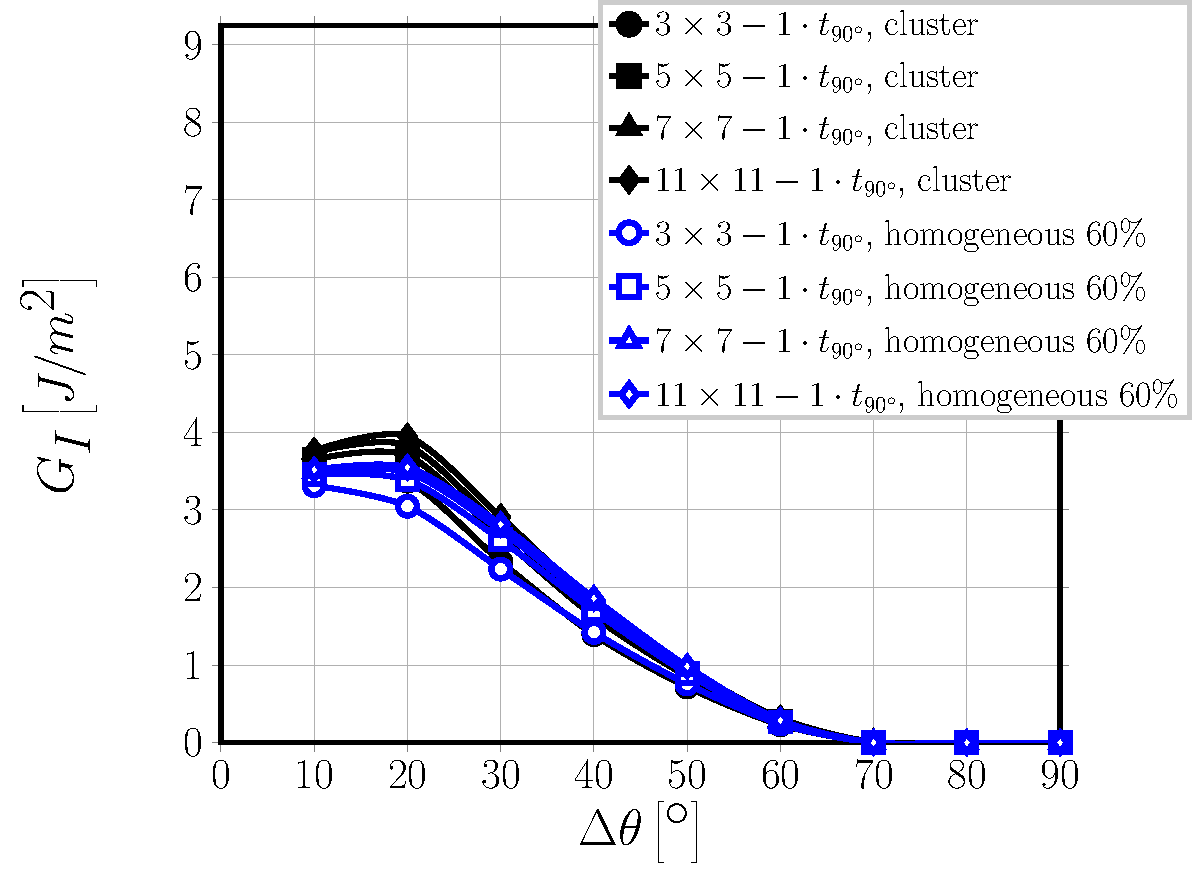
\includegraphics[width=\textwidth]{nxn-1t90-vf60-GI.pdf}
\caption{Clustering: models $n\times n-1\cdot t_{90^{\circ}}$. $V_{f}=60\%$, $\varepsilon_{x}=1\%$.}\label{fig:debonddebondGI}
\end{figure}

\begin{figure}[!h]
\centering
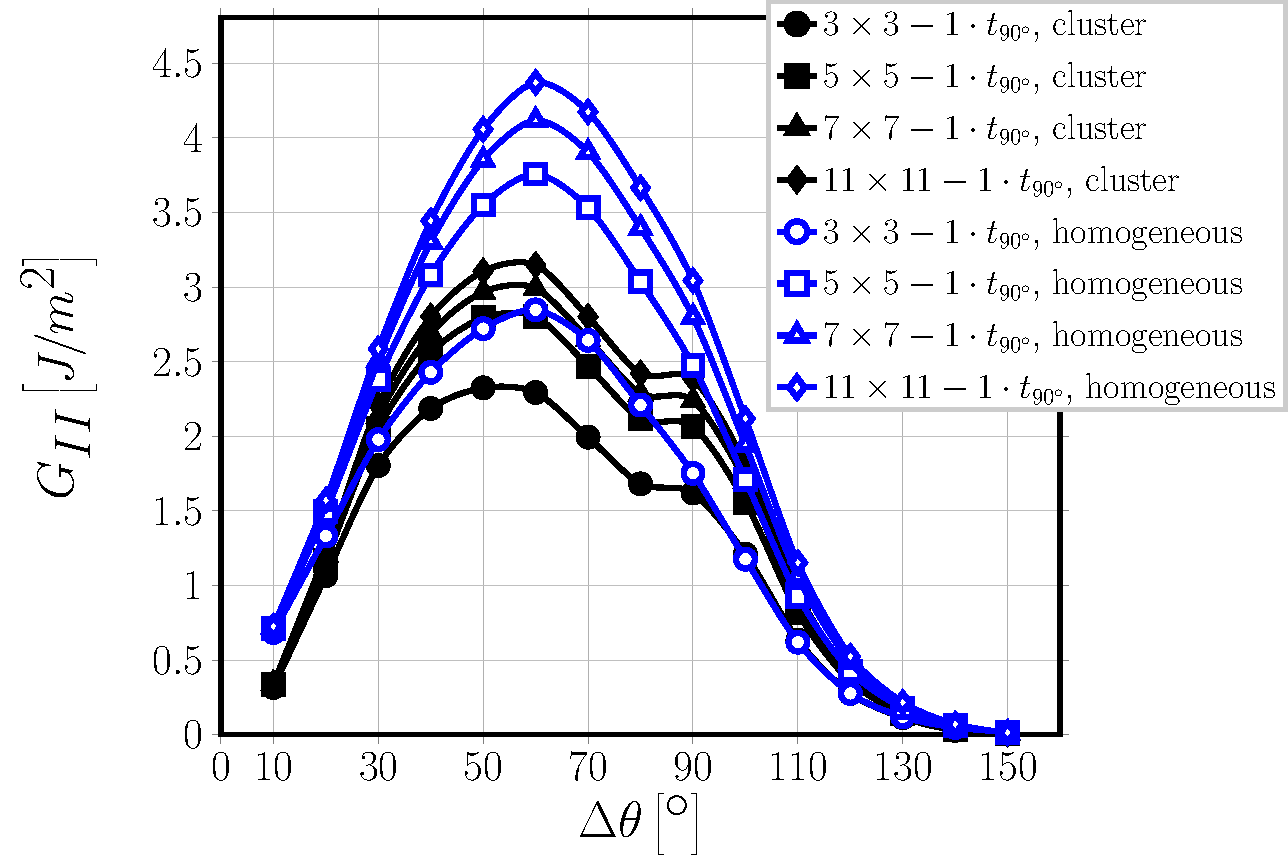
\includegraphics[width=\textwidth]{nxn-1t90-vf60-GII.pdf}
\caption{Clustering: models $n\times n-1\cdot t_{90^{\circ}}$. $V_{f}=60\%$, $\varepsilon_{x}=1\%$.}\label{fig:debonddebondGI}
\end{figure}

\section{Conclusions \& Outlook}




\section*{Acknowledgements}



\bibliography{refs}

\end{document}
